\documentclass[conference]{IEEEtran}
\IEEEoverridecommandlockouts
% The preceding line is only needed to identify funding in the first footnote. If that is unneeded, please comment it out.
\usepackage{hyperref} % For hyperlinks in the PDF
\hypersetup{
    colorlinks=true,
    linkcolor=blue,
    filecolor=magenta,
    urlcolor=cyan,
}
\usepackage{float}

\usepackage{gensymb}
\usepackage{mathtools}
\DeclarePairedDelimiter{\ceil}{\lceil}{\rceil}
\usepackage{cite}
\usepackage{amsmath,amssymb,amsfonts}
\usepackage{algorithmic}
\usepackage{graphicx}
\usepackage{textcomp}
\usepackage{xcolor}
\usepackage{multirow}
\usepackage{booktabs}
\usepackage{array}
\newcolumntype{C}[1]{>{\centering\let\newline\\\arraybackslash\hspace{0pt}}m{#1}}
\def\BibTeX{{\rm B\kern-.05em{\sc i\kern-.025em b}\kern-.08em
    T\kern-.1667em\lower.7ex\hbox{E}\kern-.125emX}}
\begin{document}


\title{Thermal-Safe Schedule Generation For
System-on-Chip Testing}

\author{Rajit Karmakar and Santanu Chattopadhyay\\
	Dept. of Electronics \& Electrical Comm. Engineering\\
		Indian Institute of Technology Kharagpur, India, Kharagpur, 721302\\
	Email: \{rajit,santanu\}@ece.iitkgp.ernet.in 
}



	\maketitle
	\begin{abstract}
		This paper presents a thermal safe test scheduling
strategy for System-on-Chip (SoC). While most of the existing
strategies rely on some approximate thermal models to avoid
the time consuming online thermal simulations, the present work
proposes to use a superposition principle-based thermal model,
which can estimate the temperature of the cores quite accurately,
yet fast, without invoking thermal simulation inside the schedule
generation process. The thermal model, along with a window-
based peak power model, has been incorporated into a Particle
Swarm Optimization (PSO) based meta search technique to
generate the test schedules. In contrast to the existing works, the
introduction of new SoC benchmarks with detailed information
regarding power and floorplan enables us to observe exact
thermal behaviors of the cores. Experimental results on these
newly proposed benchmarks show the superiority of our thermal
model over the existing ones.
	\end{abstract}
	
\textbf{\textit{Keywords---System-on-Chip; Test scheduling; Superposition
principle based thermal model; Particle Swarm Optimization; Bin
packing.}}


	\section{Introduction}
	With the increasing demand for high performance and low-
power chips, present day’s semiconductor industry is heading
towards smaller feature sizes and reduced chip area. Device
dimensions are reducing drastically, while the system designs
are becoming more and more complex. The problems related to
power and thermal issues are becoming more prominent in the
System-on-Chip (SoC) designs. Testing of such a complex chip
has become a major challenge for the test engineers. The test
mode power is often 30 times higher than the functional mode.
Not only the high power consumption, but also the high peak
temperature during testing is causing serious threat to the chip.
Due to the non-uniformity in the spatial power distribution,
the temperature may not be equal throughout the chip. High
power density of a particular core may create localized heating,
called hotspots \cite{cho2006peakaso:1}. These hotspots may lead to decrease in
the reliability of the circuit and even permanent damage of the
chip, due to thermal runaway \cite{girard2002survey}. A test engineer has to pay
special attention towards the power and thermal safety, at the
time of the development of test infrastructure of the SoC.\\
	\par
	On the other hand, shrinking product development cycle
requires to reduce the test time of the SoC. This can be
achieved via a proper scheduling of the tests for the cores.
Development of test infrastructure and schedule of a SoC under
resource, power and thermal constraints can be described as
follows. A test engineer has to (i) partition the available test
resources and allocate to the cores and (ii) decide upon the core
ordering in the test schedule, with an objective to reduce the
overall Test Application Time (TAT). Moreover, at any point
of time in the schedule, the total power consumed by all the
cores tested in parallel, must not exceed a certain pre-defined
system level power limit and the peak temperature of any core
must not violate the maximum allowable temperature limit.\\
	\par 
	To ensure the thermal-safety during testing, the temperature
of the cores, in the scheduling interval needs to be computed,
which requires online thermal simulation (i.e. at the time of
schedule generation process). However, one major drawback
of the thermal simulators like HotSpot \cite{stan2003hotspot} is their execution
time, which restricts us to invoke thermal simulators inside any
meta-search technique, that are often used to find the optimal
test schedules for the SoCs, with large number of embedded
cores. An alternative solution is to incorporate a thermal
model, which can predict the temperature of the cores, without
integrated thermal simulations. Several such approaches \cite{yu2007thermal}–
\cite{he2007heuristic} have been proposed in the literature. The RC model based
approach presented in \cite{rosinger2006thermal}, has tried to maximize the heat
dissipation through the lateral neighbourhood of the active
cores, in a test session. However, the concept of thermal
ground of the idle cores and negligible heat transfer between
the neighbouring cores does not hold, as we have reported
later in this paper, the temperature of a core largely depends
on the neighbouring cores, tested in parallel. Moreover, one
common problem with all these thermal models is, due to lots
of assumptions about the important parameters like power,
floorplan etc, these thermal models may not always predict
the temperature accurately. The exact thermal behaviour of a
chip requires the exact power profiles of the cores as well as
the accurate area and floorplan information of the chip. In the
absence of all these information of commonly used ITC’02
benchmarks, most of the work presumes some approximate
values for these parameters, which introduce inaccuracy in the
thermal behavior of the chip.\\
	\par 
	Thermal simulator like Hotspot follows linear RC thermal
model \cite{yao2011power}. The linearity of the thermal model can be exploited
using the superposition principle. The work presented in \cite{yao2011power},
tried to exploit the linearity of the Hotspot tool and used a
superposition principle based thermal model. As the CPU ex-
ecution time is the main bottleneck of the thermal simulations
during scheduling, the authors have tried to avoid invoking the
thermal simulator in the scheduling process. Instead, they have
used the HotSpot \cite{stan2003hotspot} tool to create offline thermal profiles of
the cores. These thermal profiles are used for the scheduling
purpose. This type of thermal model is fast. However, while
working with this thermal model \cite{yao2011power}, we have noticed that,
it may result in thermal violations. This, we believe, because
of neglecting the pre-schedule temperature increase of cores
due to the leakage power and also inefficient modelling of
the heating and cooling effects of the cores, which we have
discussed elaborately in Section II.\\

	\par
	To alleviate the inaccuracy of the thermal model of \cite{yao2011power}, in
this paper, we have used a more elaborate thermal model, based
on superposition principle. It uses relatively more detailed
and accurate thermal information to get an efficient, yet fast
thermal-safe test schedule. Further, the work \cite{yao2011power} do not perform
Test Access Mechanism (TAM) wire allocation to the cores.
Our work integrates TAM resource allocation with thermal-
aware test schedule generation. The integration of this fast
and accurate thermal model also aid us in designing a Particle
Swarm Optimization (PSO) \cite{kennedy2011particle} based meta-search procedure
to evolve better test schedule, exploring a large search space
of solutions. To observe the exact thermal behavior of the
cores, we have introduced a new set of SoCs, considering the
ISCAS’85, ISCAS’89 and ITC’99 benchmarks as cores, with
detail information regarding test vectors, area, floorplan, dy-
namic and leakage powers. Experimental results on the newly
formed SoCs show that our model estimates temperature better
than \cite{yao2011power}, hence assures thermal safety of the test schedule more
efficiently.\\

	\par
	Rest of the paper is organised as follows. Section II
presents the proposed superposition principle based thermal
model. The basic requirements to develop test infrastructure
and the test scheduling strategy is described in Section III.
Section IV presents a new set of SoC benchmarks and also
the experimental results on the proposed benchmarks. Finally
Section V draws the conclusion of the paper.\\


	\section{Superposition Principal Based Thermal Model}
	
	In this section, we have proposed a superposition principle
based thermal model. It takes the help of the linearity of the
thermal model of HotSpot and uses offline HotSpot \cite{stan2003hotspot} thermal
simulations for each core in different possible conditions
and creates thermal databases for all those conditions. These
database information are used for the scheduling purpose. It
helps us to generate a thermal safe test schedule much faster
than the techniques that use online Hotspot simulations. To get
the exact thermal behavior of a core, it is very much important
to observe the different conditions, which can change the
temperature of a core. Figure 1 summarises different possible
conditions of temperature dependency between cores.


\hypertarget{model}{\begin{figure}[ht]
    \center
   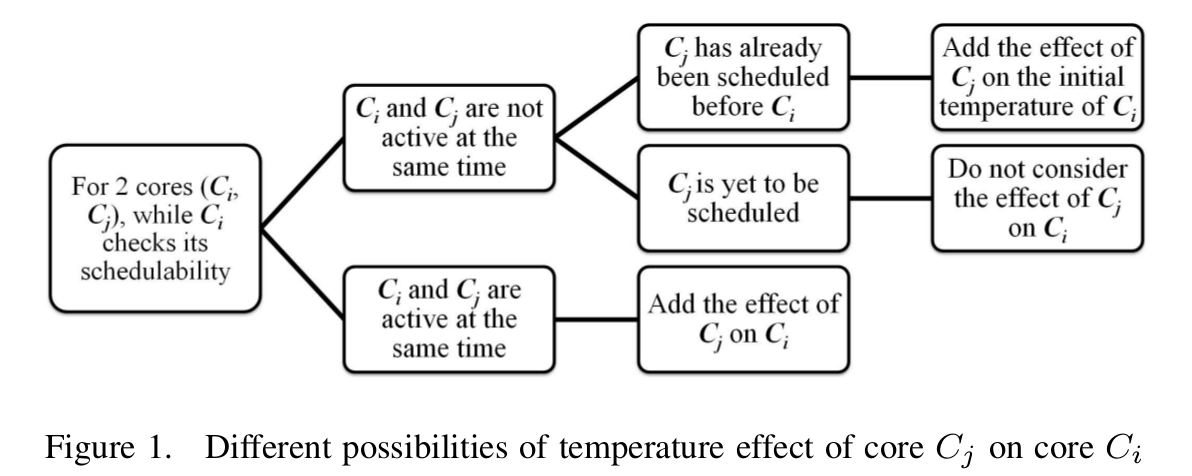
\includegraphics[width=\columnwidth]{2.png}
\end{figure}}


	\par
	The temperature of a core C$_{i}$ can increase due to the
following activities.\\
\hspace*{0.5cm}$\bullet$ Before C$_{i}$ starts its testing, its initial temperature increases due
to its leakage power consumption (Figure 2(a)).\\
\hspace*{0.5cm}$\bullet$ During the period of testing of the core C$_{i}$ , its temperature
increases (Figure 2(b)).\\
\hspace*{0.5cm}$\bullet$ If any numbers of other cores C$_{j}$ (1 $\leq$ j $\leq$ N)(j $\neq$ i) are tested
in parallel with C$_{i}$ , due to the lateral spreading of heat from C$_{j}$ ,
the temperature of C$_{i}$ increases (Figure 2(b)). \\
\hspace*{0.5cm}$\bullet$ Initial temperature of C$_{i}$ increases due to the effect of all the
cores which have already been scheduled before C$_{i}$ starts its
testing (Figure 2(c)).\\

 
	\par 
	Figure 2 shows some simulation results on SoC k10
(details of the SoC has been mentioned in Section IV-A)
to depict the exact thermal behavior of core 1 in different
conditions. Figure 2(a) shows the increase in the initial
temperature of core 1 due to the leakage power consumption
before it starts its testing in SoC k10. Figure 2(b) shows the
extra heating effect on core 1, if it is tested in parallel with core
2. Figure 2(c) shows the effect of the already scheduled cores
on the initial temperature of a core chosen to be scheduled
next. When core 1 is idle and core 2 is being tested, because
of lateral heat spreading from core 2, the initial temperature
of core 1 increases by 10\degree C. If core 1 starts its test just after
core 2 has finished, the initial temperature of core 1 should
be 10\degree C more than its normal initial temperature. However, if
core 1 starts its test after a certain time interval, in that time
gap, its initial temperature reduces towards its normal initial
temperature. Depending upon the scheduling position of any
core, the thermal model should be able to handle all these
conditions and generate a test schedule that does not violate the
thermal constraint. The objective of the superposition principle
based thermal model is to sum up the individual effects of
other cores on the temperature of a particular core, based
on its ordering in the test schedule. The operation of our
superposition principle based thermal model can be described
by the following steps.\\


	\par
	\textbf{\textit{Step I:}} For each core C$_{i}$ (1 $\leq$ I $\leq$ N), calculate the
increase in the initial temperature, due to leakage power
consumption. Create a thermal database of it.\\


\vspace{8 mm}\begin{figure}[ht]
    \centering
   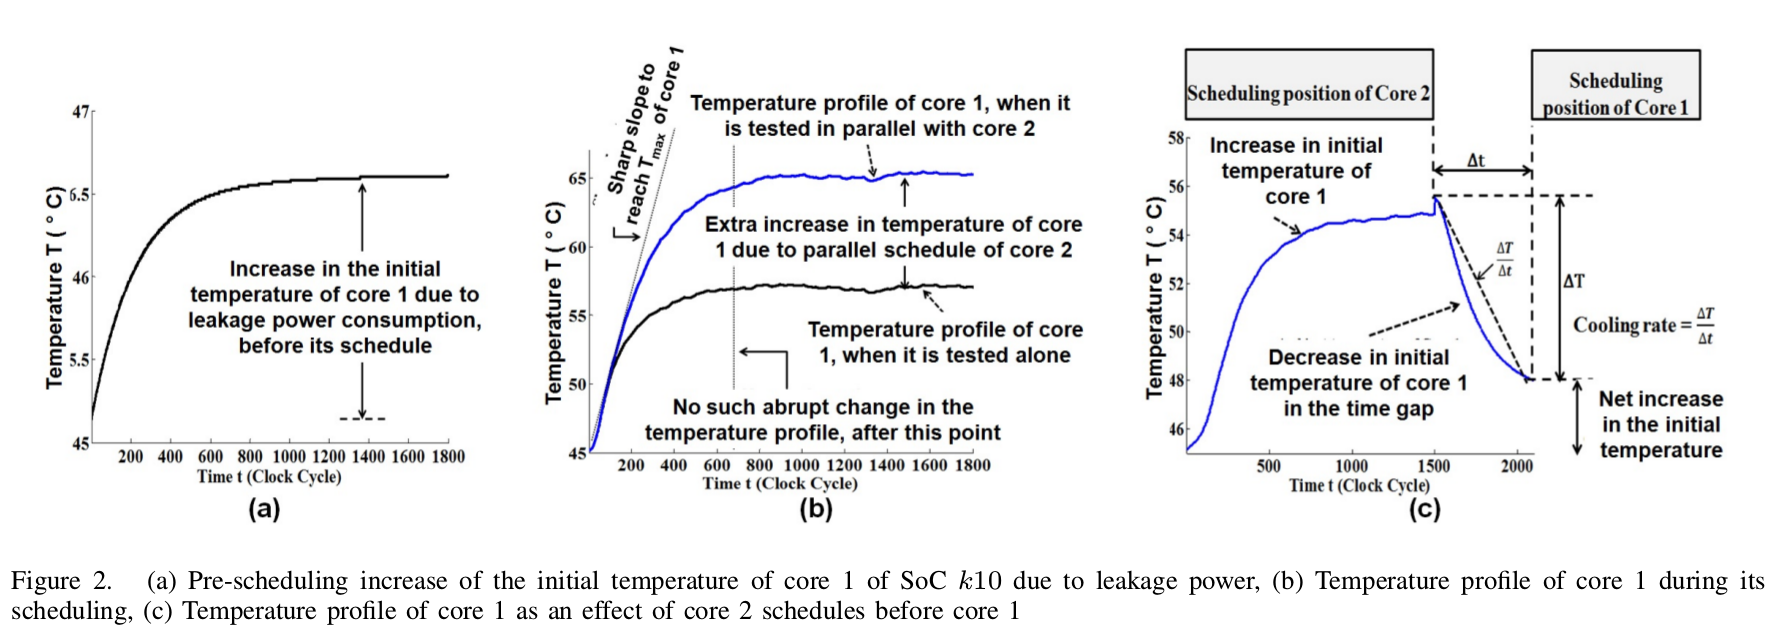
\includegraphics[width=160 mm,scale=0.5]{3.png}
\end{figure}




	\par
	\textbf{\textit{Step II:}} For each core C$_{i}$ (1 $\leq$ I $\leq$ N), calculate its
temperature rise, when it is tested alone. Then, calculate the
extra increase in the temperature of C$_{i}$ , due to the core C$_{j}$ (1 $\leq$
j $\leq$ N )(I $\neq$ j), when C$_{j}$ tests in parallel with C$_{i}$ . This
extra increase in the temperature of C$_{i}$ is calculated for each
C$_{j}$ separately. Create a thermal database of it. Superposition
principle is applied to calculate the actual temperature increase
of core C$_{i}$ , considering the cores, tested in parallel with C$_{i}$.\\

	\par
	\textbf{\textit{Step III:}} For each core C$_{i}$ (1 $\leq$ i $\leq$ N), calculate its initial
temperature increase, due to the core C$_{j}$ (1 $\leq$ j $\leq$ N)(i $\neq$
j), which is scheduled prior to C$_{i}$. Let us assume, the initial
temperature increase is T$_{1}$. Calculate the cooling rate for the
combination of C$_{i}$ and C$_{j}$, from the slope of the temperature
decrease curve, as mentioned in Figure 2(c). Although the
temperature decrease portion of the curve is not exactly linear,
still a linear prediction of this portion of the curve can be a
good approximation to calculate the simplified cooling rate. If
the time gap is $\Delta$t and the temperature decrease in $\Delta$t time
is $\Delta$T, then, cooling rate can be calculated as

\begin{equation}
\textit{Cooling rate} = \frac{\Delta T}{\Delta t}\\
\end{equation}
 

    \par
	The net increase in the initial temperature of C$_{i}$ is (T$_{1}$ - $\Delta$T). This is carried out for each C$_{j}$, corresponding to each
C$_{i}$. Two thermal databases store all these information. Super-
position principle is applied to calculate the actual increase in
the temperature of C$_{i}$, considering all such C$_{j}$.\\


	\par
	The superposition principle based thermal model, proposed
in \cite{yao2011power}, neglects the scenario of the pre-schedule increase in
the initial temperature of a core, because of leakage power
consumption. Moreover, to take care of the heating effect of
the pre-scheduled cores and to introduce a cool down period
after a test completion, the work \cite{yao2011power} proposes to make the
power profiles of the finished cores to zero, for the rest of
the schedule duration. However, the thermal simulation of
each core is carried out offline and its scheduling position is
unknown, until all the cores have been scheduled. Apparently,
it is not clear from \cite{yao2011power}, that, how long one should carry on \\\\\\\\\\\\\\\\\\\\\\\\\\\\\\\\ the
offline thermal simulation for each core. As the waiting time
of a core before it starts its testing is unknown and can only
be determined by the scheduling process, the total test time of
all the cores cannot be predicted beforehand. This makes the
thermal model more complex. On the other hand, our thermal
model handles the pre-schedule heating effects of a core more
efficiently, hence estimates the temperature more accurately.\\




	\section{Test Infrastructure Development and Test
Scheduling}

	\textbf{\textit{Problem Formulation}}\\
	
	\par
	Suppose a SoC with N cores C$_{1}$, C$_{2}$...C$_{N}$ is to be tested
with a maximum of W$_{max}$ TAM resources, a maximum power
limit P$_{max}$, and a maximum temperature limit T$_{max}$. The
test scheduling problem is to allocate TAM resources and test
times to the cores so that, the total test application time (TAT)
is minimized, while the power consumption during testing
remains under P$_{max}$ and the maximum temperature of any
core does not cross the temperature upper bound of T$_{max}$.\\

\textbf{\textit{A. Test Infrastructure Development}}\\

	\par
	The basic requirements of test infrastructure development
of a SoC under resource, power and thermal constraints are to
consider a power model to estimate the test mode power of the
cores and a thermal model to estimate the temperature of the
cores during testing. Power profile of each core is required to
check power validation at each point of the schedule, while
selecting test parallelism between the cores. Calculation of
the temperature of the cores also requires the power profile
information of the cores, while a thermal model is used to
avoid the time consuming online thermal simulations.

$\bullet$ \hspace{1 cm} \textbf{\textit{Power Profile Generation:}}

	\par
	We have used a window-based peak power model \cite{karmakar2015window} to
estimate the test mode power of the cores. For this purpose,
we have first calculated the cycle-accurate power profile of
each core. Cycle-accurate power profile of a core can be
estimated using the information of the transition counts in
the wrapper chains in every clock cycle and the dynamic
power consumption of the core. Average transition (ATR) is
calculated for the total test time of the core. Dynamic power
(DP) consumption of a core can be obtained using Synopsys
Design Vision Report Power Compiler tool \cite{lettnin2004synthesis} as mentioned
in the Table I in Section IV-A. If the transition in i$^{th}$ cycle
is TR$_{i}$, the cycle-accurate power of the i$^{th}$ cycle (CAP$_{i}$) can
be estimated as

\begin{equation}
CAP_{i} = \frac{TR_{i}}{ATR} \times DP\\
\end{equation}

From this cycle-accurate power profile, we calculate the
window-based peak power profile for each core by partitioning
the total test time of the core into some smaller sized time
windows and considering a single peak power in that interval to
represent the power value for that interval. A suitable window-
size results in an efficient balance between the scheduling
complexity of the cycle-accurate power model \cite{samii2008cycle} and the
power-overestimation of the global peak power model \cite{chou1997scheduling}.
These window-based power profiles of all the cores are used
in the next steps of power validity and estimation of thermal
profiles.


$\bullet$ \hspace{1 cm} \textbf{\textit{Thermal database creation:}}

	\par
	After generating the power profile of each core, we cre-
ate offline thermal databases from these power profiles
and the floorplan of the chip, using offline Hotspot ther-
mal simulations. Four such databases are created, con-
sidering different thermal conditions between the cores.
\textit{Thermal\_Database\_1(TD1)} stores the values of the ini-
tial temperature rise, due to the leakage power consump-
tion of each core. \textit{Thermal\_Database\_2(TD2)} stores the
temperature values of self testing as well as parallel test-
ing. The increase in the initial temperature of a core, be-
cause of the previously scheduled cores, are stored using
two thermal databases, \textit{Thermal\_Database\_3(TD3)} and
\textit{Thermal\_Database\_4(TD4)}. The procedures of thermal
database generations are mentioned next in \textit{Procedure\_TD1},
\textit{Procedure\_TD2}, \textit{Procedure\_TD3} and \textit{Procedure\_TD4}.\\

$\bullet$ \textbf{\textit{Procedure\_TD1 (Thermal\_Database\_1 (TD1)):}}

	\par
	1) For all the cores C$_{i}$(1 $\leq$ i $\leq$ N), create power profile
P$_{leakagei}$, by considering leakage power of C$_{i}$ and zero
power value of other cores.\\
\hspace*{.33 cm}2) Calculate the maximum temperature, T leakage i from the
transient and steady state responses of C$_{i}$ and update TD1.\\


$\bullet$ \textbf{\textit{Procedure\_TD2 (Thermal\_Database\_2 (TD2)):}}

	\par
	1) For all the cores C$_{i}$(1 $\leq$ i $\leq$ N), create power profile
P$_{selfi}$, by considering dynamic power of C$_{i}$ for the clock
cycles to test C$_{i}$ and leakage power values of other cores.\\
\hspace*{.33 cm}2) Calculate the maximum temperature, T$_{selfi}$ from the tran-
sient and steady state responses of C$_{i}$ and update TD2.\\
\hspace*{.33 cm}3) For each core C$_{j}$(1 $\leq$ j $\leq$ N)(j $\neq$ i), create power profile
P$_{parallelij}$ , by considering the dynamic power of C$_{i}$ and C$_{j}$
for the clock cycles required to test C$_{i}$ and leakage powers
for all other cores C$_{k}$(k $\neq$ j $\neq$ i).\\
\hspace*{.33 cm}4) Calculate the maximum temperature, T$_{parallelij}$, from the
transient and steady state responses of C$_{i}$.\\
\hspace*{.33 cm}5) T$_{extraij}$ = T$_{parallelij}$ −T$_{selfi}$ and update T$_{extraij}$ in TD2.\\

$\bullet$ \textbf{\textit{Procedure\_TD3 (Thermal\_Database\_3 (TD3)):}}

	\par
	1) For all the cores C$_{i}$(1 $\leq$ i $\leq$ N), corresponding to the core
C$_{j}$ (1 $\leq$ j $\leq$ N)(j $\neq$ i), create pre-schedule power profile
P$_{preschedule1ij}$, by considering dynamic power of C$_{j}$ and
leakage powers for all other cores C$_{k}$(k $\neq$ j), including C$_{i}$
for the clock cycles required to test C$_{j}$.\\
\hspace*{.33 cm}2) Calculate the maximum temperature, T$_{preschedule1ij}$ of C$_{i}$,
from the transient and steady state responses, update TD3.\\

$\bullet$ \textbf{\textit{Procedure\_TD4 (Thermal\_Database\_4 (TD4)):}}

	\par
	1) For all the cores C$_{i}$(1 $\leq$ i $\leq$ N), corresponding to the
core C$_{j}$(1 $\leq$ j $\leq$ N)(j $\neq$ i), create pre-schedule power
profile P$_{preschedule2ij}$, by considering dynamic power of C$_{j}$
for the clock cycles required to test C$_{j}$ , leakage powers of
C$_{j}$ for next 2000 number of clock cycles and leakage power
for all other cores C$_{k}$(k $\neq$ j), including C$_{i}$ for the entire
time period.\\
\hspace*{.33 cm}2) Calculate the final temperature, T$_{preschedule2ij}$ of C$_{i}$ , from
the transient and steady state responses of C$_{i}$, update TD4.\\


	\par
	In \textit{Procedure\_TD1}, T$_{leakagei}$ is the maximum increase in
the initial temperature of C$_{i}$, due to leakage power consump-
tion. In \textit{Procedure\_TD2}, T$_{selfi}$ is the temperature increase
of core C$_{i}$, when no other cores are tested in parallel with C$_{i}$.
T$_{parallelij}$ is the maximum increase in temperature of C$_{i}$, when
it is tested in parallel with C$_{j}$. T$_{extraij}$ is the extra increase
in the temperature of C$_{i}$, as an effect of parallel testing of
C$_{j}$ with C$_{i}$. In \textit{Procedure\_TD3}, T$_{preschedule1ij}$ calculates
the maximum increase in the initial temperature of C$_{i}$, as an
effect of the earlier scheduling of C$_{j}$. In \textit{Procedure\_TD4}, we
allow C$_{i}$ to cool down towards its normal initial temperature
for 2000 clock cycles. T$_{preschedule2ij}$ is the initial temperature
of C$_{i}$ after 2000 clock cycles. The cooling rate of C$_{i}$ for the
combination of C$_{i}$ and C$_{j}$ can be calculated as


\begin{equation}
Cooling \hspace{.1cm} Rate \left(CR_{ij}\right) = \frac{\left(T_{preschedule1ij}-T_{preschedule2ij}\right)}{2000}\\
\end{equation}

We can calculate the actual reduction in the initial temperature
of C$_{i}$, by multiplying CR$_{ij}$ with the time gap (TG) between
the end time of C$_{j}$ and start time of C$_{i}$. The net increase in
the initial temperature of C$_{i}$, because of the earlier scheduling
of C$_{j}$, can be calculated as

\begin{equation}
Net \hspace{.1cm} Initial \hspace{.1cm} Increase = T_{preschedule1ij}-\left(CR_{ij} \times TG\right)
\end{equation}

\textbf{\textit{B. Particle Swarm Optimization Guided Test Scheduling}}\\

	\par
	In this step, we generate a valid power and thermal-safe test
schedule. Rectangular bin packing approach is used to partition
and allocate test resources to the cores and to decide the core
order in the test schedule. Each core C$_{i}$(1 $\leq$ i $\leq$ N ) is repre-
sented by a set of wrapper configurations R$_{i}$. The test resource
requirement of core C$_{i}$ with J$^{th}$ wrapper configuration can be
represented by a rectangle whose height and width represent
allocated TAM width (w$_{ij}$) and the corresponding test time
(T(w$_{ij}$)) respectively. To get a schedule for the full SoC, the
rectangles are to be packed into a bin of fixed height (W$_{max}$),
so that the TAT (width of the bin) is minimized. As the bin
packing problem is NP-Hard \cite{iyengar2002using}, we have utilized a Particle
Swarm Optimization based meta search technique to solve the
scheduling problem. In PSO, each particle corresponds to a
solution to the optimization problem being solved. Any PSO
formulation involves choosing a proper representation of the
particles, their fitness calculation, and defining an evolution
policy. Let, the number of cores in the SoC be N and
the maximum number of rectangles for any core is M. Let
B = $\ceil*{log_{2}M}$. A particle consists of N $\times$ B number of bits.
First B bits identify the test rectangle selected for the first
core, second B bits for the second core, and so on. Figure 3
shows a simple particle with N = 4 and B = 4. In this case,
test rectangles 9, 2, 8 and 13 are selected for cores 1, 2, 3 and
4 respectively. Particles evolve over the generations guided by
self \textit{(lbest)} and group-intelligence \textit{(gbest)}, and also via their
inertia. A \textit{replace} operator attempts to align a particle with its
\textit{pbest} and the \textit{gbest} particles, with some probability. For bit
position \textit{i} of a particle, the bit is replaced by the corresponding
bit of \textit{pbest} and \textit{gbest} particles with probability $\alpha$ and $\beta$
respectively to evolve a new particle. Fitness of a particle is
equal to the total test time (TAT) of the SoC after scheduling
the test rectangles using the algorithm \textit{Schedule\_Rectangles}.

\hypertarget{model}{\begin{figure}[ht]
    \center
   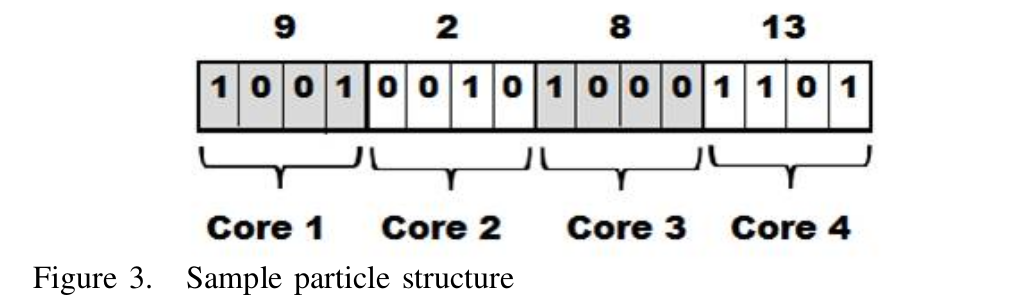
\includegraphics[width=\columnwidth]{4.png}
\end{figure}}


The Schedule Rectangles algorithm takes as input the
rectangle set corresponding to the particle, the maximum TAM
width W$_{max}$, the maximum power limit P$_{max}$ and the max-
imum allowable temperature T$_{max}$. It performs a scheduling
of the rectangles, honouring the constraints that at no instant
of time, the total TAM width requirement exceeds W$_{max}$, and
the instantaneous power value does not exceed P$_{max}$. Also
the maximum temperature of individual cores does not exceed
T$_{max}$. A \textit{Power\_Violation\_Checker(PVC)} checks whether
there is any power violation during scheduling. If at any partic-
ular point in the schedule, a core does not respect PVC, it does
not get the permission to get scheduled at that point. Similarly,
a \textit{Thermal\_Violation\_Checker(TVC)} checks whether any
core is violating thermal budget or not. TVC checks the
scheduling position of a core and uses the superposition
principle to add different thermal values from \textit{TD1, TD2,
TD3 and TD4,} corresponding to that core to calculate the
exact temperature of the core. \textit{BP, ATW} and \textit{PT} keep track
of the scheduling points, corresponding resource availability at
those points and the power values at \textit{BPs} respectively, while
\textit{TT} notes the temperature of each core. As the till unscheduled
cores get scheduled, the list \textit{BP, ATW, PT} and \textit{TT} also get
updated. The bin packing procedure also needs to prioritize
the next unscheduled rectangle to be selected for packing
(scheduling). For this purpose the rectangles are sorted on their
area values (TAM width(\textit{w}) × test time(\textit{T})) in a descending
order. The break-point list \textit{BP} is scanned from the minimum
to the maximum value. When the rectangles corresponding to
all the cores have been scheduled, the maximum end time of
the testing of all the cores gives the total test application time.
The algorithm to produce the schedule is presented next.

\hypertarget{model}{\begin{figure}[ht]
    \center
   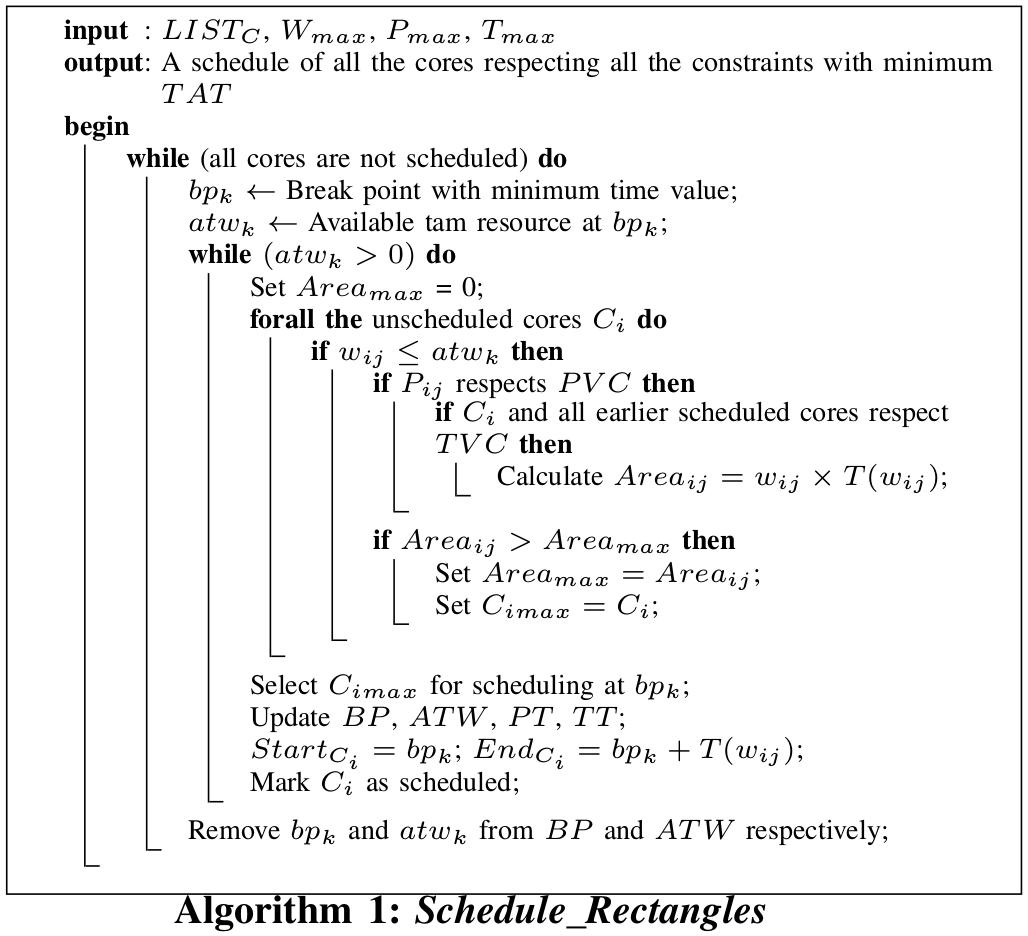
\includegraphics[width=\columnwidth]{5.png}
\end{figure}}



\section{Experimental Results and Discussions}

\textbf{\textit{A. Experimental Setup}}
\par
Fewer details of the traditional ITC’02 SoC benchmarks
have motivated us to form new SoCs with detail information
to observe the exact thermal behaviour of them. We have
developed two SoCs, named k10 and k25 having 10 and
25 cores respectively, using ITC’99, ISCAS 89 and ISCAS
85 circuits. From the benchmark suites mentioned above, a
number of cores have been designed as follows.

$\bullet$ Each circuit description in \textit{Verilog} format (.v) has been taken
as input and mapped to the Faraday 90nm standard cell library
\cite{karmakar2016thermal}. The circuits are synthesized using the \textit{Synopsys Design
Vision} Compiler \cite{lettnin2004synthesis} to generate gate-level netlist from the
\textit{Verilog} design description.

$\bullet$ All the flip-flops are replaced by scan flip-flops using the
\textit{Synopsys DFT} Compiler for the testability purpose.

$\bullet$ Multiple scan chains are inserted to reduce the TAT.

$\bullet$ Dynamic and leakage powers are extracted from the \textit{Synopsys
Design Vision Report Power} tool \cite{lettnin2004synthesis}.

$\bullet$ Area of the cores are calculated using the \textit{Cadence Encounter}
tool \cite{davis2008big}.

$\bullet$ Exact floorplan of the SoCs are calculated using the Floorplan-
ning tool \textit{Blobb} \cite{chan2004practical} , \cite{kapur2013test} and \textit{Plottool}. The empty spaces in
the floorplan are packed with the zero power boxes to make it
compatible with the HotSpot tool. The packing of the empty
spaces with zero power boxes are done using a C program.

$\bullet$ Test patterns are generated using the Synopsys \textit{TetraMax
ATPG} tool \cite{weed2006chip}.

	\par
	Table I reports the value of the different parameters
of different circuits, that we have obtained using the above
mentioned tools. The components of two newly formed SoCs
k10 and k25 are also mentioned in this table.


\textbf{\textit{B. Experimental Results}}\\

1) \textbf{\textit{Thermal-Aware Test Scheduling:}} In this section, we
present the results of our experimentation under resources,
power and thermal constraints, for different SoCs. Superpo-
sition principle based thermal model, along with the window-
based peak power model, has been considered to guide PSO
based power and thermal-aware test scheduling strategy. Table
II shows the results on two newly formed SoCs k10 and k25.
We have shown the simulation results for W$_{max}$ = 64 and 56,
for both the SoCs and varied the P$_{max}$ and T$_{max}$ values. It may
be observed that, if we increase the P$_{max}$ and T$_{max}$ values,
TAT (in clock cycles) gets reduced. Also, for a particular P$_{max}$
value, if we increase T$_{max}$ value, TAT gradually reduces.
This happens as with the relaxation of power and thermal
constraints, TAT can be minimized further. It may be noted
that in some cases increase in the T$_{max}$ value does not really
help to reduce the TAT value further. It is because of the fact
that the SoC has already reached its saturation TAT in that
temperature range. Variation in the temperature does not have
any impact on the TAT, in that temperature range. However,
direct comparison of our work with other related thermal-aware
test scheduling works is not possible, as they assume their own
power profiles and different floorplans.


	\par
	2) \textbf{\textit{Comparison Between Thermal Models:}} In this part, we
focus on the comparison between our proposed thermal model
and the thermal model proposed in \cite{yao2011power}. Our main objective in
comparison between the two thermal models is to find the
minimum temperature budget at which the thermal models
can produce test schedules and then checking the thermal
validation of the obtained schedules, using the Hotspot thermal
simulations. To check the quality of the two thermal models,
we have tried to fit the thermal model proposed in \cite{yao2011power} in our
TAM constrained test scheduling strategy and then compare
with our proposed thermal model.

	\par
	Table III presents the minimum allowable temperature
values to get a valid test schedule (T$_{max}$), for both the thermal
models and their corresponding maximum temperature values
obtained from the post-schedule Hotspot simulations (T$_{out}$).
It may be noted that, using the thermal model proposed in
\cite{yao2011power}, we are able to generate test schedules at 70\degree C and 78\degree C for



\begin{table}[H]
\caption{INFORMATION OF THE CORES OF NEWLY FORMED SOCS}
\begin{tabular}{|c|c|c|c|c|c|c|c|}
\hline
\multirow{3}{*}{\textbf{\begin{tabular}[c]{@{}c@{}}Circuit\\ name\end{tabular}}} & \multirow{3}{*}{\textbf{\begin{tabular}[c]{@{}c@{}}DP\\ (mW)\end{tabular}}} & \multirow{3}{*}{\textbf{\begin{tabular}[c]{@{}c@{}}LP\\ (uW)\end{tabular}}} & \multirow{3}{*}{\textbf{\begin{tabular}[c]{@{}c@{}}No.\\ Test \\ Vector\end{tabular}}} & \multirow{3}{*}{\textbf{\begin{tabular}[c]{@{}c@{}}No.\\ Scan\\ Chain\end{tabular}}} & \multirow{3}{*}{\textbf{\begin{tabular}[c]{@{}c@{}}Max\\ Scan\\ length\end{tabular}}} & \multicolumn{2}{c|}{\textbf{\begin{tabular}[c]{@{}c@{}}No of copies\\ in SoC\end{tabular}}} \\ \cline{7-8} 
 &  &  &  &  &  & \multirow{2}{*}{\textbf{k10}} & \multirow{2}{*}{\textbf{k25}} \\
 &  &  &  &  &  &  &  \\ 
\hline
s38584 & 9.15 & 315.57 & 146 & 32 & 45 & 2 & 2 \\ 
\hline
s38417 & 4.60 & 311.45 & 100 & 32 & 55 & 2 & 0 \\ 
\hline
s35932 & 10.27 & 282.44 & 64 & 32 & 54 & 0 & 2 \\ 
\hline
s15850 & 3.05 & 128.62 & 131 & 16 & 34 & 1 & 0 \\ 
\hline
s13207 & 1.91 & 116.48 & 273 & 16 & 41 & 0 & 1 \\ 
\hline
s9234 & 1.23 & 71.08 & 147 & 4 & 54 & 1 & 2 \\ 
\hline
s5378 & 0.72 & 35.09 & 124 & 4 & 46 & 0 & 2 \\ 
\hline
b22 & 4.35 & 218.53 & 1501 & 46 & 15 & 0 & 1 \\ 
\hline
b21 & 2.55 & 143.38 & 711 & 16 & 31 & 1 & 2 \\ 
\hline
b17 & 3.67 & 346.39 & 1477 & 46 & 31 & 0 & 3 \\ 
\hline
b15 & 1.18 & 120.60 & 457 & 16 & 29 & 2 & 2 \\ 
\hline
b14 & 1.32 & 68.12 & 737 & 4 & 62 & 1 & 1 \\ 
\hline
c7552 & 3.59 & 38.45 & 219 & 0 & 0 & 0 & 3 \\ 
\hline
c5315 & 2.29 & 27.89 & 123 & 0 & 0 & 0 & 2 \\ 
\hline
c1908 & 0.95 & 7.52 & 119 & 0 & 0 & 0 & 1 \\ 
\hline
c499 & 0.01 & 1.12 & 52 & 0 & 0 & 0 & 1 \\ 
\hline
\end{tabular}
\end{table}




\begin{table}[H]
\caption{Variation in Test Application Time (TAT) for
Different SoCs with the Variation of $_{max}$ and T$_{max}$}
\begin{tabular}{|c|c|c|c|c|c|}
\hline
\multirow{2}{*}{k10} & \multirow{2}{*}{\begin{tabular}[c]{@{}c@{}}T$_{max}$\\ (\degree C)\end{tabular}} & \begin{tabular}[c]{@{}c@{}}P$_{max}$\\ = 1.3 Watt\end{tabular} & \begin{tabular}[c]{@{}c@{}}P$_{max}$\\ = 1.5 Watt\end{tabular} & \begin{tabular}[c]{@{}c@{}}P$_{max}$\\ = 2 Watt\end{tabular} & \begin{tabular}[c]{@{}c@{}}P$_{max}$\\ = 5 Watt\end{tabular} \\ 
\cline{3-6} 
 &  & TAT & TAT & TAT & TAT \\ 
 \hline
\multirow{5}{*}{\begin{tabular}[c]{@{}c@{}}W$_{max}$\\ = 64\end{tabular}} & 72 & 43154 & 42494 & 42365 & 42365 \\ \cline{2-6} 
 & 80 & 41424 & 41388 & 41347 & 40924 \\ 
 \cline{2-6} 
 & 90 & 39349 & 37875 & 37875 & 37875 \\ 
 \cline{2-6} 
 & 100 & 39349 & 35880 & 34810 & 34459 \\ 
 \cline{2-6} 
 & 110 & 39349 & 35732 & 34268 & 34021 \\ 
 \hline
\multirow{5}{*}{\begin{tabular}[c]{@{}c@{}}W$_{max}$\\ = 56\end{tabular}} & 72 & 50285 & 50285 & 50285 & 49010 \\ \cline{2-6} 
 & 80 & 43530 & 42424 & 42424 & 42424 \\ 
 \cline{2-6} 
 & 90 & 43530 & 39672 & 39672 & 39672 \\ 
 \cline{2-6} 
 & 100 & 42300 & 39672 & 39672 & 39672 \\ 
 \cline{2-6} 
 & 110 & 42300 & 39672 & 38936 & 38936 \\ 
 \hline
\multirow{2}{*}{k25} & \multirow{2}{*}{\begin{tabular}[c]{@{}c@{}}T$_{max}$\\ (\degree C)\end{tabular}} & \begin{tabular}[c]{@{}c@{}}P$_{max}$\\ = 2.7 Watt\end{tabular} & \begin{tabular}[c]{@{}c@{}}P$_{max}$\\ = 3 Watt\end{tabular} & \begin{tabular}[c]{@{}c@{}}P$_{max}$\\ = 3.5 Watt\end{tabular} & \begin{tabular}[c]{@{}c@{}}P$_{max}$\\ = 4.5 Watt\end{tabular} \\ 
\cline{3-6} 
 &  & TAT & TAT & TAT & TAT \\ 
 \hline
\multirow{4}{*}{\begin{tabular}[c]{@{}c@{}}W$_{max}$\\ = 64\end{tabular}} & 82 & 171142 & 169876 & 169869 & 169684 \\ 
\cline{2-6} 
 & 90 & 170578 & 169562 & 169146 & 169101 \\ 
 \cline{2-6} 
 & 100 & 169513 & 169101 & 168982 & 168778 \\ 
 \cline{2-6} 
 & 110 & 168698 & 168602 & 168602 & 168602 \\ 
 \hline
\multirow{4}{*}{\begin{tabular}[c]{@{}c@{}}W$_{max}$\\ = 56\end{tabular}} & 82 & 196567 & 196567 & 193613 & 192163 \\ 
\cline{2-6} 
 & 90 & 195710 & 193202 & 192494 & 192050 \\ 
 \cline{2-6} 
 & 100 & 192494 & 191894 & 191276 & 191276 \\ 
 \cline{2-6} 
 & 110 & 191814 & 191644 & 191276 & 191276 \\ 
 \hline
\end{tabular}
\end{table}

the SoCs k10 and k25 respectively. However, while using
our proposed thermal model, we can get test schedules at
minimum temperature levels of 72\degree C and 82\degree C, for these two
SoCs respectively. Our thermal model is unable to produce test
schedules for any thermal budget lower than that. For example,
when fed with 70\degree C as T$_{max}$ value, our tool does not produce
any schedule for k10. It could work successfully only with a
limit of 72\degree C. The actual thermal simulations show this limit
to be a bit pessimistic as the Hotspot results range between
70.66\degree C and 71.92\degree C. This, we believe, has occurred due to
the simplified time overlapping model that has been used in our
model. In our model, if there is a small overlap in the scheduled
test times of two cores, it has been taken as a complete overlap
of their test durations, which is probably not accurate for most
of the cases. However, this pessimistic assumption could result
in thermally valid test schedules.

	\par
	Although, the thermal model presented in \cite{yao2011power} produces
valid test schedules with a lower temperature limit than our
thermal model, it does not always ensure thermal safe test
schedule. It violates thermal limits in most of the cases. On
the other hand, our thermal model violates the thermal limit for
none of the cases. This is because our proposed thermal model
takes care of the pre-scheduled heating effects of the cores
more efficiently by considering both the temperature increase
due to the leakage power and doing proper estimation of the
heating and cooling effects of the already scheduled cores with
more accuracy. This shows the efficiency of our thermal model.



\begin{table}[H]
\caption{Comparison of Validation of Test schedule of Our
Thermal Model with the Thermal Model Prsented in \cite{yao2011power}}
\begin{tabular}{|C{0.5cm}|C{0.5cm}|C{0.5cm}|C{0.5cm}|c|c|C{0.5cm}|c|C{0.5cm}|}
\hline
\multirow{2}{*}{\begin{tabular}[c]{@{}c@{}}SoC\\ name\end{tabular}} & \multirow{2}{*}{W$_{max}$} &  & \multicolumn{3}{c|}{Thermal Model {[}8{]}} & \multicolumn{3}{c|}{Our Thermal Model} \\ 
\cline{3-9} 
 &  & \begin{tabular}[c]{@{}c@{}}P$_{max}$\\ (Watt)\end{tabular} & \begin{tabular}[c]{@{}c@{}}T$_{max}$\\ (\degree C)\end{tabular} & \begin{tabular}[c]{@{}c@{}}T$_{out}$\\ (\degree C)\end{tabular} & \begin{tabular}[c]{@{}c@{}}Viola-\\ tion\end{tabular} & \begin{tabular}[c]{@{}c@{}}T$_{max}$\\ (\degree C)\end{tabular} & \begin{tabular}[c]{@{}c@{}}T$_{out}$\\ (\degree C)\end{tabular} & \begin{tabular}[c]{@{}c@{}}Viola-\\ tion\end{tabular} \\ 
 \hline
\multirow{12}{*}{k10} & \multirow{4}{*}{32} & 1.3 & 70 & 70.74 & \textbf{Yes} & 72 & 70.74 & No \\ 
\cline{3-9} 
 &  & 1.5 & 70 & 71.56 & \textbf{Yes} & 72 & 70.74 & No \\ 
 \cline{3-9} 
 &  & 2 & 70 & 70.74 & \textbf{Yes} & 72 & 70.74 & No \\ 
 \cline{3-9} 
 &  & 5 & 70 & 71.3 & \textbf{Yes} & 72 & 71.81 & No \\ 
 \cline{2-9} 
 & \multirow{4}{*}{48} & 1.3 & 70 & 70.79 & \textbf{Yes} & 72 & 70.66 & No \\ 
 \cline{3-9} 
 &  & 1.5 & 70 & 70.8 & \textbf{Yes} & 72 & 70.66 & No \\ 
 \cline{3-9} 
 &  & 2 & 70 & 70.86 & \textbf{Yes} & 72 & 70.66 & No \\ 
 \cline{3-9} 
 &  & 5 & 70 & 70.86 & \textbf{Yes} & 72 & 70.66 & No \\ 
 \cline{2-9} 
 & \multirow{4}{*}{64} & 1.3 & 70 & 71.2 & \textbf{Yes} & 72 & 70.66 & No \\ 
 \cline{3-9} 
 &  & 1.5 & 70 & 70.91 & \textbf{Yes} & 72 & 70.91 & No \\ 
 \cline{3-9} 
 &  & 2 & 70 & 71.32 & \textbf{Yes} & 72 & 71.1 & No \\ 
 \cline{3-9} 
 &  & 5 & 70 & 70.91 & \textbf{Yes} & 72 & 70.66 & No \\ 
 \hline
\multirow{12}{*}{k25} & \multirow{4}{*}{32} & 2.7 & 78 & 77.94 & No & 82 & 78.27 & No \\ 
\cline{3-9} 
 &  & 3 & 78 & 79.05 & \textbf{Yes} & 82 & 78.13 & No \\ 
 \cline{3-9} 
 &  & 3.5 & 78 & 79.88 & \textbf{Yes} & 82 & 79.2 & No \\ 
 \cline{3-9} 
 &  & 4.5 & 78 & 78.09 & \textbf{Yes} & 82 & 77.5 & No \\ 
 \cline{2-9} 
 & \multirow{4}{*}{48} & 2.7 & 78 & 78.14 & \textbf{Yes} & 82 & 78.72 & No \\ 
 \cline{3-9} 
 &  & 3 & 78 & 78.14 & \textbf{Yes} & 82 & 77.15 & No \\ 
 \cline{3-9} 
 &  & 3.5 & 78 & 77.8 & No & 82 & 77.52 & No \\ 
 \cline{3-9} 
 &  & 4.5 & 78 & 77.84 & No & 82 & 77.77 & No \\ 
 \cline{2-9} 
 & \multirow{4}{*}{64} & 2.7 & 78 & 76.77 & No & 82 & 77.12 & No \\ 
 \cline{3-9} 
 &  & 3 & 78 & 76.42 & No & 82 & 77.94 & No \\ 
 \cline{3-9} 
 &  & 3.5 & 78 & 76.72 & No & 82 & 77.34 & No \\ 
 \cline{3-9} 
 &  & 4.5 & 78 & 76.95 & No & 82 & 77.18 & No \\ 
 \hline
\end{tabular}
\end{table}


\section{Conclusion}
In this paper, a new superposition principle based fast ther-
mal model, which is capable of estimating temperature with
accuracy, has been proposed. The thermal model along with a
window-based peak power model, has been incorporated into
a PSO based formulation to select the test rectangles for the
cores and scheduling them using a 3-D bin-packing approach.
A new set of SoC benchmarks with detail information has been
used to get exact thermal effects of the cores at the time of
generation of thermal-aware test schedule using the proposed
method. The proposed approach can generate efficient test
schedules without violating power and thermal constraints.


\bibliography{assignment} 
\bibliographystyle{ieeetr}

\end{document}
